\chapter{Aktivitätsdiagramm}

In diesem Kapitel erfolgt die Erarbeitung der Aktion 'Standort mit neuen Fahrzeugen anlegen' in Form von Aktivitätsdiagrammen. Da hierbei von einer vollständig leeren Datenbasis ausgegangen werden soll, muss jedoch die Aktion aufgegliedert werden. Die Unteraktionen 'Standort anlegen', 'Fahrzeug anlegen' und letztendlich 'Fahrzteug einem Standort zuordnen' müssen somit voneinander getrennt betrachtet werden. 

\section{Pseudo-Code}

-to be continued-

\section{Diagramme}

\newpage

\subsection{Standort anlegen}

\begin{figure}[!ht]
    \centering
    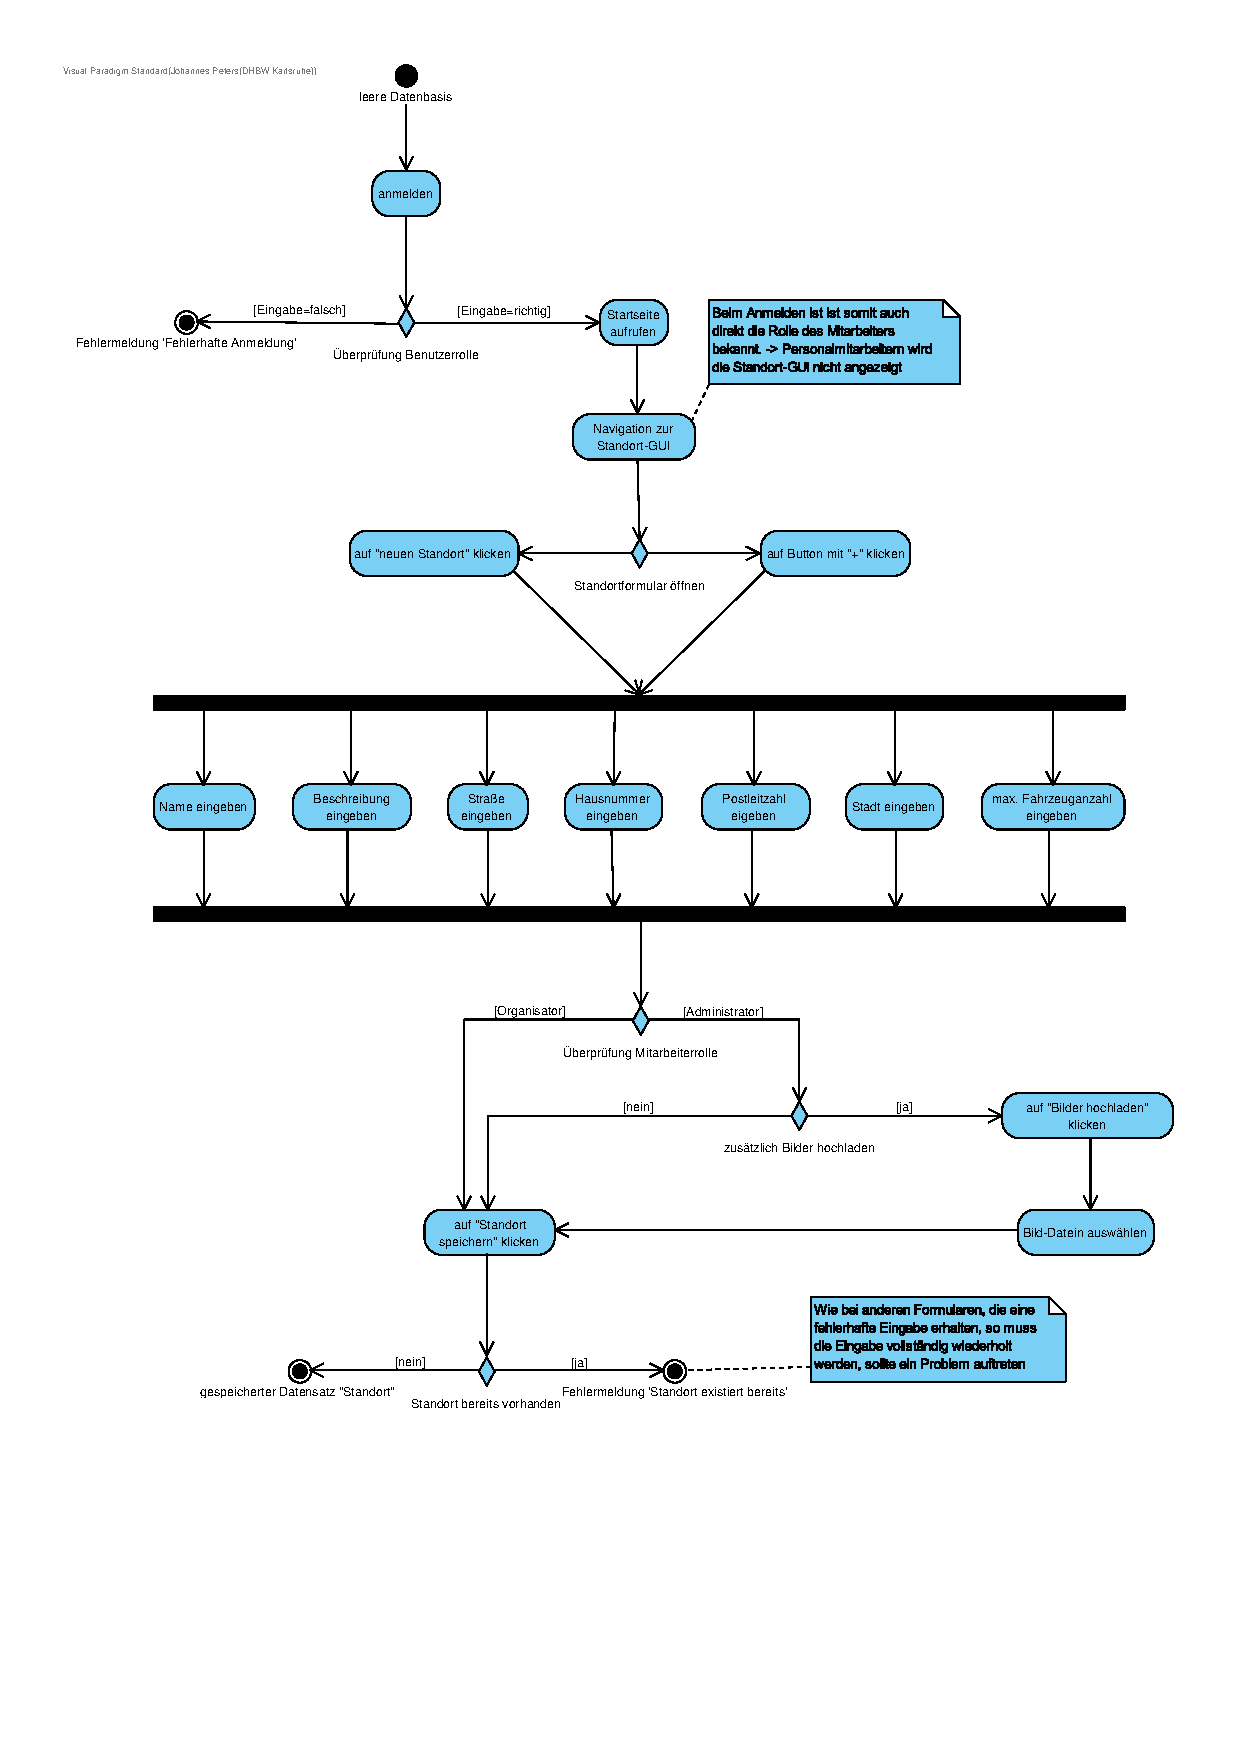
\includegraphics[width=\textwidth, height=\textheight-3cm, trim = 0cm 3cm 0cm 0cm]{Bilder/Diagramme/AD_Standort_anlegen.pdf}
    \caption{Aktivitätsdiagramm: Standort anlegen}
    \label{img:ad_standort}
\end{figure}

Wie bei jeder anderen auf dem System ausgeführten Aktion muss auch beim Anlegen eines neuen Standorts zuerst eine Anmeldung vollzogen werden. Sobald ein Mitarbeiter im System angemeldet ist stehen mittels seines Benutzerprofils auch die Rechte des Nutzers griffbereit. Personalmitarbeiter soll es nicht möglich sein, Standorte anzulegen oder andere Aktionen mit solchen Datensätzen auszuführen, sodass diesen Mitarbeitern eine andere Benutzeroberfläche gezeigt wird wie den Organisatoren und Administratoren. 


Nachdem zu der entsprechenden GUI navigiert wurde und der Mitarbeiter einen neuen Standort anlegen möchte, gibt es zwei Möglichkeiten zum entsprechenden Eingabeformular zu gelangen. Um für die Mitarbeiter, deren IT-Kenntnisse teils mangelhaft sind, mehrere Vorschläge darzustellen gibt es einmal den offensichtlichen Text-Button mit 'neuen Standort anlegen', für die etwas bewanderten Mitarbeiter, zusätzlich einen '+'-Button. Sobald sich das Eingabeformular geöffnet hat, müssen die Felder ausgefüllt werden. 


In welcher Reihenfolge dies ausgeführt wird, ist irrelevant, weshalb im Diagramm diese Aktionen auf parallel dargestellt werden. Sobald alle Texteingaben abgeschlossen wurden, besteht noch die Option Bilder vom Standort hochzuladen, sozusagen ein Titelbild für den Detaileintrag des Standorts. Das Hochladen von Bildern dürfen nur die Administratoren ausführen, sodass zuerst eine Rollenabfrage stattfindet. Sollte ein Administrator diesen Standort anlegen, so wird ihm die Möglichkeit angezeigt und sollte er Bilder hinzufügen möchten, kann er über einen 'Standard-File-Choose-Dialog' Bilder von seinem Computer auswählen und in das Programm laden. Sofern dies erledigt wurde, oder auch nicht, ist es möglich den neuen Standorteintrag zu speichern. 


Bevor der Standort gespeichert wird, erfolgt die Überprüfung, ob dieser Standort bereits vorhanden ist. Sollte das Ergebnis negativ sein, wird der Standort gespeichert. Ist jedoch in der Planung oder Organisation ein Fehler aufgetreten und der Standort exisitiert bereits, erscheint eine Fehlermeldung und die Aktion wird abgebrochen. An sich hätte man im Diagramm anstelle des Endzustandes 'Fehlermeldung' auch eine Schleife einbauen können, die solange läuft wie die Eingabe inkorrekt ist oder bis die Aktion händisch abgebrochen wird. In diesem Fall wird jedoch davon ausgegangen, dass allein auf Basis der Funktionsart eines Eingabeformulars die Eigabefelder geleert werden und die Eingabe wiederholt werden muss. Außer der Abfrage, ob der Standort bereits existiert, findet keine andere logische Überprüfung statt. Sofern sich die Adresse nicht doppelt wird der Datensatz gespeichert. Sollte die Fehlermeldung erscheinen, ist es auch sehr unwahrscheinlich, dass der Mitarbeiter ein zweites Mal die Erstellung des Standortes versucht. 
\newpage

\subsection{Fahrzeug anlegen}

\newpage

\subsection{Fahrzeug einem Standort zuordnen}


\chapter{To-Do}

AnalyseKlassenDiagramm: 
- Abändern: Fahrzeug kann 0 oder 1 Standort zugeordnet sein

Sequenzdiagramm:
- Erstellen: Pseudo-Code ausstehend
- Erstellen: Diagramm für neuen Kunden anlegen